%! TEX root = diss.tex
\documentclass[../diss.tex]{subfiles}
\chapter{Implementation}

% NOTE: Multiprocessor => shared memory. Use term "parallel computer" instead

% Introduction:
% * TODO: change fig 2.1 to have cloud of "graph data.csv" that interact with
%   "input graph"
% * Refer to figure 2.1, go into some more depth on interface to Parallel
%   system simulation:
%   * You create Worker implementation with access to ...., then pass
%     description to manager, specify number of workers, topology to use, num
%     computation phases, etc.
% * _Intrdc the different components, and then start going into detail in ind. subsecs_

% Some "practices used/software dev.? chapter":
% * Weekly meetings, log book, 

% Graph datasets:
% * California road networks:
%   * freely-available, consisten format, real-life road network
% * Random graphs:
%   * To satisyf req. of different n
%   * Erdos-Renyi graph, but modified to be fully-connected, trick to get same properties
%     with formula for creating $p$
%   *  python library used
% * Graph reader
%   * adjacency matrix and also neighbourhood list for Dijkstra's algorithm
% Graph datasets {{{
\section{Graph datasets}%
\label{sec:Graph datasets}

To run the algorithms, we need graphs as input. Since one important usage of \ac{APSP}
is route-planning, I used a dataset of the Californian road-network. This dataset was
initially used in \citep{graph-dataset} and has been made available on the author's
website\footnote{\url{https://www.cs.utah.edu/~lifeifei/SpatialDataset.htm}}.
% TODO: add plot of the dataset as a figure, using the python script...
This graph was used to prove that practical problems can quickly be solved on my
simulated parallel system, as long as graph compression is used.
However, for evaluation I needed graphs of various sizes, so these were generated
randomly.

\subsection{Random graph generation}%
\label{sub:Random graph generation}

% TODO: information on Erdos-Renyi graphs in prepreration chapter...

I chose to use Erd{\"o}s-Renyi graphs because they have previously been used in
evaluation of \ac{APSP} algorithms.
% TODO: cite https://core.ac.uk/download/pdf/81103122.pdf
%            https://www.researchgate.net/publication/47842024_A_Parallelization_of_Dijkstra%27s_Shortest_Path_Algorithm
I have tried to fit the parameters as closely to the real-world graph datasets as possible. There are many characteristics of a graph, such as vertex- and edge-connectivity,
betweenness centrality, clustering coefficient, and average distances. However,
trying to generate new graphs with similar values for all of these metrics quickly
becomes a difficult problem. I have therefore only tried to replicate the metric,
\textit{average vertex degree}, which should have some correlation to the mentioned
metrics. I also want the random graphs to be fully-connected, as most road-networks
are. In the $G(n,p)$ random-graph model, the graph is constructed by starting with a
set of $n$ vertices, and then independently include every possible edge $e$ with
% (TODO: citation???)
probability $p$. This makes the edges follow the binomial distribution:
\begin{equation}
    \textrm{deg}(v) \sim \textrm{Binomial}(n-1,p)
\end{equation}
with the average degree being $(n-1)p$. However, by instead starting with a
\textit{circular graph} and including each remaining edge independently with
probability 
\begin{equation}
    p=\frac{\textrm{desired average degree} - 2}{n - 3},
\end{equation}
we get a fully-connected graph where the average degree is as desired.
% TODO: proof in appendix...
I chose the desired average degree based on the Californian road-network, which is
2.061. However, since we will be using the compressed graph (see \autoref{sec:Graph compression}), I used the average vertex degree of the compressed California graph instead,
which was 2.945. In \autoref{fig:example-graph-random}, I have plotted an
example graph generated through this method. I then generated ? graphs of various
sizes, from 10 nodes to 700 nodes for use in evaluation. %TODO: how many?

\begin{table}
    \centering
    \begin{tabular}{|c|c|}
        \hline
        \textbf{Location} & \textbf{Average vertex degree} \\
        \hline
        San-Francisco (SF) &  2.549 \\
        \hline
        North-America (NA) & 2.038 \\
        \hline
        ? (OL) & 2.305 \\
        \hline
        California (cal) & 2.061 \\
        \hline
        ? (TG) & 2.614 \\
        \hline
    \end{tabular}%
    \caption[Caption]{Average vertex degree for various road-network datasets\footnotemark.}%
    \label{tab:vertex-degree}
\end{table}

\footnotetext{These values were computed using the TODO??? method in \texttt{GraphReader}.}

\begin{figure}
\begin{center}
    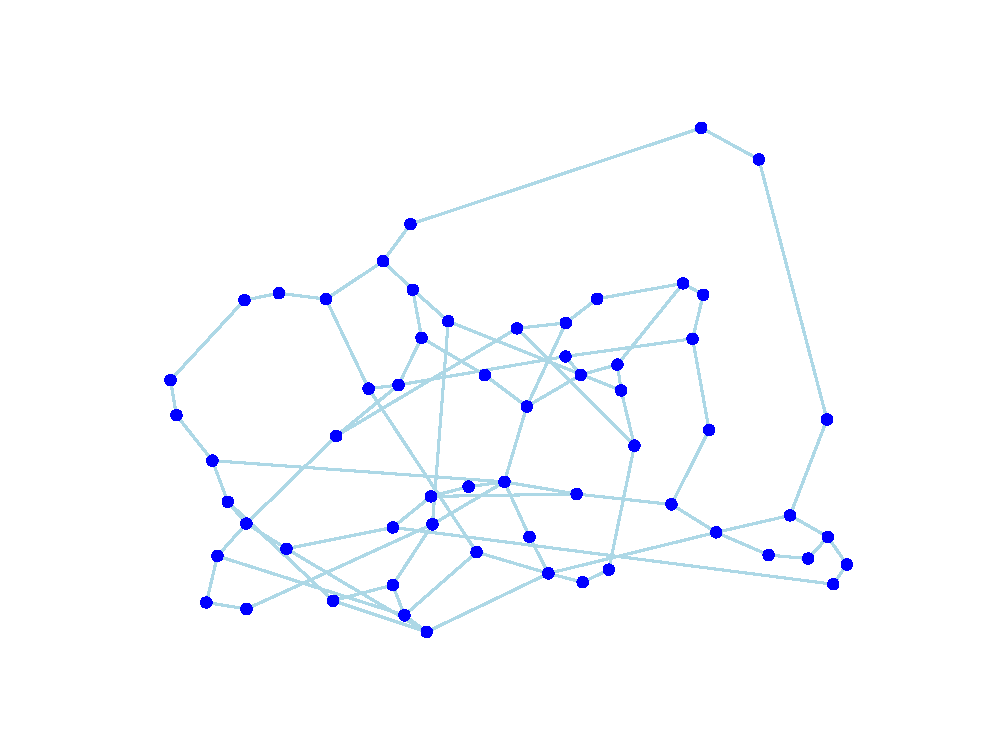
\includegraphics[scale=.7]{figs/plots/example-graph.eps}
\end{center}
\caption[Caption]{A visualisation of a graph generated with the modified
    Erd{\"o}s-Renyi model. The graph has $n=60$ vertices, and the length of the edges
correspond to their weight\footnotemark.}%
\label{fig:example-graph-random}%
\end{figure}

\addtocounter{footnote}{-1}
\footnotetext{The graph was visualised using the \texttt{ForceAtlas2} library in python. See TODO}

% \begin{algorithm}
%     \caption{Fully-connected random graph with specific average degree}%
%     \label{alg:random-graph}
%     \KwData{$n$, avg\_degree}
%     \KwResult{$G=(V,E)$}
%
%     $G \leftarrow (\textrm{set of } n \textrm{ vertices}, \emptyset)$
%
%     \For{vertices $v_{i}, v_{i+1}$}{
%         $E \leftarrow E \cup (v_{i}, v_{i+1}, w), \textrm{ where } w \sim \textrm{Uniform}[0,1]$
%     }
%     $E \leftarrow E \cup (v_{0}, v_{n-1}, w), \textrm{ where } w \sim \textrm{Uniform}[0,1]$
%
%     Not finished....
%
% \end{algorithm}


% }}}

% Simulation of a distributed memory multiprocessor:
% * Introduction:
% *   Overview of the components in bigger UML diagram, and comments on their interaction
% * TODO: create the above diagram first, and then realise what **more than below**
%         aspects to explain...
% * Memory model (?)
%   * explain design decision behind Map : (label : String) -> (value : Number)
%   * ...
% * Work management
%   * _By now, reader should know communication manager modifies memory when flush_
%   * Diagram of how work is simulated in parallel fashion, 8 blocks at a time
%   * Use Java's executor service to avoid thread management overhead
% * Worker factory
%   * Use of reflection, so can allow arbitrary description to be passed and can still
%     crete the new worker objects that can be managed
% * Timing analysis
%   * implemented as decorators for the system simulation
%   * Explain equations for how MIMD simulated (stalling bc. wait, latency+bandwidth etc.
%   * Repating computation measures, cache misses effect, possible bc.
%     seperation, mask read writes to ensure same computation done,
%     goal is more accurate eval
% Simulation of a distributed memory multiprocessor {{{
\section{Simulation of a distributed memory multiprocessor}%
\label{sec:Simulation of a distributed memory multiprocessor}

% }}}

% APSP via repeated matrix-squaring
% * Can abbriviate as MatSquare or something
% * Start with top-down explanation, what happens when do A^2 and same for pred. matrix
% * Then explain the driver code, why this number of iterations etc.
% * Then explain generalized fox otto algorithm, noting special case for pred. matrix
% * Explain FoxOtto (explain predecessor functionality and edge-case,
%   generalized version, pseudo-code, diagram of memory movement can go in preparation)
% * Explain driver code, and its complexity?
% * As explain, also use a simple graph as an example, going through as you do the
%   general explanation
% APSP via repeated matrix-squaring {{{
\section{APSP via repeated matrix-squaring}%
\label{sec:APSP via repeated matrix-squaring}

The \emph{\acl{MatSquare}} algorithm, which I will abbreviate as \emph{\acs{MatSquare}},
is an algorithm. \acused{MatSquare}
By using \ac{MatSquare}, we can ...


% Notes from reserach-and-planning diary:
% **Problem with generalized FoxOtto**: 
% In the general version, we first started the multiplication by iterating from
% the top of the submatrix (see diagram in notes for $C_{10,6}$ for instance).
% However, this causes problems for the predecessor values because of the initial
% conditions. Consider the scenario for $C_{10,6}$ where want to compute path 10
% -> 10. Whenever we get to $k=10$, we would not assign predecessor because of
% exemption condition (which is necessary, otherwise we get other bugs). And at
% this point ($k=10$) we discover path of length 0. However, because of the
% generalization, we start with $k=8$ (ref. to diagram), so we find another path
% of longer length, and when we get to $k=10$, we optimize the path, but leave
% the predecessor as it was for the longer path because of the exemption
% condition. One fix is to save the initial "dist" and not use $\infty$ every
% time. Another option is making sure we start with $k=10$ when running algo i.e.
% being consistent with non-general version. That way, we immediately relax
% distance to 0 and keep the initial predecessor, this.j (or read("P") which is
% same thing). This is the option I went for, and is the reasoning behind the `m`
% loop and then modifying `iter`.
%
% * In `CountingMemoryController`, we assume
% that each PE only sends data to **one** other PE, but this is NOT CHECKED
% anywhere. However, it is enforced in underlying memory controller that each PE
% can only receive from **one** other PE, which is not equivilant, but in _most
% cases_ (all PE do the same thing) causes the above assumption to hold.

% }}}

% Graph compression:
% * The algorithm for this, and explain all the edge cases, **with diagrams**
% * Also simple graph to use as an example
% * Also a section for the expected asymptotic speed-up referencing random graph generation
% Graph compression {{{
\section{Graph compression}%
\label{sec:Graph compression}

% }}}

% vim: foldmethod=marker
